\documentclass[11pt]{beamer}
\newcommand{\R}{\mathbb{R}}
\newcommand{\C}{\mathbb{C}}
\newcommand{\Z}{\mathbb{Z}}
\newcommand{\N}{\mathbb{N}}
\DeclareMathOperator*{\argmin}{arg\,min}
\DeclareMathOperator{\cotan}{cotan}
\DeclareMathOperator{\sinc}{sinc}
\DeclareMathOperator{\Tr}{Tr}
\DeclareMathOperator{\tr}{tr}
\DeclareMathOperator{\Gram}{Gram}
\DeclareMathOperator{\diag}{diag}
\newcommand{\lp}{\left(}
  \newcommand{\rp}{\right)}
\usepackage{blkarray}
\usepackage{multirow}
\usepackage{framed,fancybox}
\usepackage{tikz}
% \usepackage{algorithm2e}
% \usepackage{algorithmic}
\usepackage{float}
\usepackage{framed}
% \usepackage{ulem}
\usetikzlibrary{shapes,arrows}

\newcommand{\lela}{\left \langle}
  \newcommand{\rira}{\right \rangle}
\newcommand{\norm}[1]{\left\lVert#1\right\rVert}
\newcommand{\abs}[1]{\left|#1\right|}

\usepackage{tikz}
\usetikzlibrary{shapes,arrows}
\usepackage[french,english]{babel}
\usepackage[utf8]{inputenc}
\usepackage[T1]{fontenc}
\usepackage{lmodern}
% \usepackage{common}
\usepackage{amsmath,amsfonts,amssymb}
% \usepackage{overpic,boxedminipage}
\usepackage{hyperref}
\usetheme{Warsaw}
\setbeamercolor*{block body alerted}{bg= blue!10}
\setbeamercolor*{block title alerted}{bg= blue!50}
% \usefonttheme{professionalfonts}
\setbeamertemplate{navigation symbols}{}
\setbeamertemplate{headline}{}
\setbeamertemplate{footline}{}
% \setbeamertemplate{blocks}[rounded][shadow=false]
\title[iX_Blue]{Optimisation de trajectoire pour la navigation bathymétrique}
\author{Kieran Delamotte, Carlo de Franchis, David Gontier, Antoine Levitt, François Madiot, Carlo Marcati}
\date{SEME, Vendredi 16 Janvier 2015}
\institute{Sujet proposé par Jérémy Nicola, iXBlue}
% \institute{CEA, DAM, DIF\\Collaboration avec Marc Torrent}
\newcommand{\loja}{\L{}ojasiewicz\xspace}
\begin{document}

\frame{\titlepage}

\frame{\tableofcontents}
\AtBeginSection[]{
  \begin{frame}{Sommaire}
    \tableofcontents[currentsection, hideothersubsections]
  \end{frame}
}

\section{Présentation du problème}
%\subsection{Contexte}
%\frame{
%  \frametitle{Positionnement}
%  \begin{itemize}
%  \item Activité principale de iXBlue : conception de système de
%    positionnement pour le pétrolier
%  \item Interféromètre à base de fibre optique : donne les
%    accélérations selon les six degrés de liberté
%    \begin{center}
%    \resizebox{.3\textwidth}{!}{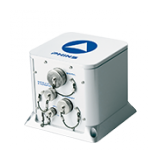
\includegraphics{Images/phins}}
%    \resizebox{.5\textwidth}{!}{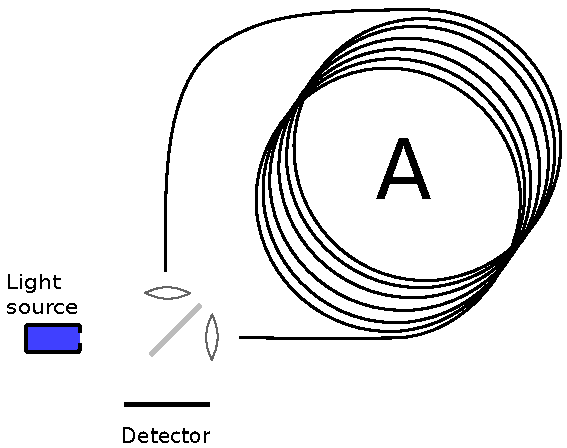
\includegraphics{Images/interferometre}}
%  \end{center}
%  \end{itemize}
%
%}

%%%%%%%%%%%%%%%%%%%%%%%%%

\frame{
  \frametitle{Problématique du sous-marin}
  

 
  $\bullet$ Un \textcolor{red}{sous-marin} se déplace à \textcolor{blue}{profondeur constante} (pas de GPS).\\
  $\bullet$ \textcolor{red}{Problème :} A cause des imprécisions de ses appareils de mesure, et de la dérive, il peut se perdre.\\
  $\bullet$ \textcolor{red}{Idée} : il peut se \textcolor{red}{recaler} en mesurant le fond marin, et en comparant avec des cartes bathymétriques
  
\begin{center}
    \resizebox{.35\textwidth}{!}{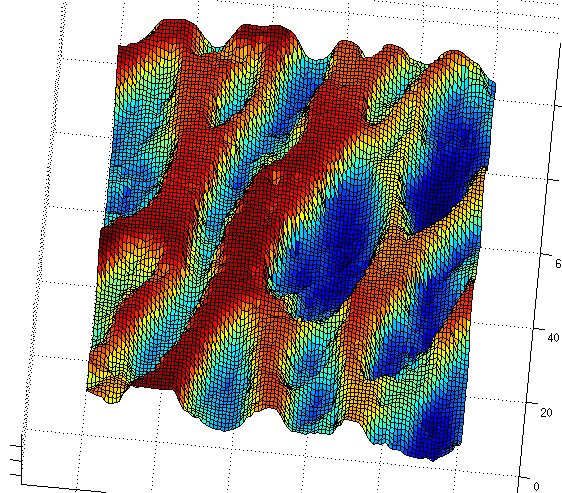
\includegraphics{Images/bathy.png}}
  \end{center}
  
  \textcolor{red}{Question :} \\
  \begin{center}
  	Quelles sont les trajectoires qui permettent un recalage précis~?
	\end{center}
}

%%%%%%%%%%%%%%%%%%%%%%%%%
\begin{frame}

\frametitle{Présentation du problème}


\textcolor{red}{Sous-marin parfait} : 
\begin{itemize}
	\item connait parfaitement la trajectoire de $A$ à $B$.
	\item calcule parfaitement $(v_x(t), v_y(t), h(t))$.
\end{itemize}


\begin{figure}[!h]
\begin{center}
	\begin{tikzpicture}[scale =1]

	%% Boite trajectoire
	\draw (0,0) rectangle (7, 6);
	
	% A et B
	\node at (1, 3.8) {$A$};
	\node at (6, 2.8) {$B$};
	
	% Obstacle
	\foreach \r in {0.1, 0.2, 0.3, 0.5, 0.8}
	{
		\draw (4, 1.5) circle (\r);
	}
		
	\draw[line width=1.5]  (1, 3.5) -- (4, 1.5) -- (6, 2.5);
	\only<1> \shade[ball color=red] (1,3.5) circle (.15);
	\only<2> \shade[ball color=red] (4,1.5) circle (.15);
	\only<3> \shade[ball color=red] (6,2.5) circle (.15);
	

	% temps t
	\only <2> {\draw (10, -0.1) -- (10, 5.8); \node at (10.2, 5.7) {$t$};}
	
	%% Boite vx
	\draw[->] (8, 4) -> (11, 4); 	\draw[->] (8, 4) -> (8, 5.8);	
	\node at (8.3, 5.5) {$v_x$}; \node at (11.2, 4) {$t$};
	
	\only<2-> \draw[red, line width=1.2] (8, 5) -- (10, 5);
	\only<3> \draw[red, line width=1.2] (10,5.4) -- (11, 5.4);
	
	%% Boite vy
	\draw[->] (8, 2) -> (11, 2); 	\draw[->] (8, 2) -> (8, 3.8);
	\node at (8.3, 3.5) {$v_y$}; \node at (11.2, 2) {$t$};
	
	\only<2-> \draw[red, line width=1.2] (8, 2.5) -- (10, 2.5);
	\only<3> \draw[red, line width=1.2] (10,3.4) -- (11, 3.4);
	
	%% Boite h
	\draw[->] (8, 0) -> (11, 0); 	\draw[->] (8, 0) -> (8, 1.8);
	\node at (8.3, 1.5) {$h$}; \node at (11.2, 0) {$t$};
	
	\only<2-> \draw[red, line width=1.2] (8, 0.2) -- (9.4, 0.2);
	\only<2-> \draw[red, line width=1.2]  (9.4,0.2) .. controls (9.7,0.2) and (9.8,1.5) .. (10,1.5);
	\only<3> \draw[red, line width=1.2]  (10,1.5) .. controls (10.2,1.5) and (10.3,0.2) .. (10.6,0.2);
	\only<3> \draw[red, line width=1.2] (10.6, 0.2) -- (11, 0.2);


\end{tikzpicture}
\end{center}
\end{figure}


\end{frame}

\begin{frame}

\frametitle{Présentation du problème}


\textcolor{red}{Sous-marin réel} : (\textbf{va suivre la même trajectoire})
\begin{itemize}
	\item connait parfaitement $A$, et la carte de fond.
	\item Il mesure $(\widetilde{v_x}(t), \widetilde{v_y}(t), \widetilde{h}(t)) = (v_x(t), v_y(t), h(t)) + (e_{v_x}(t), e_{v_y}(t) , e_h(t))$.
	\item \textcolor{red}{But : estimer où est $B$ !}
\end{itemize}

\vspace{-1.5em}

\begin{figure}[!h]
\begin{center}
	\begin{tikzpicture}[scale =1]

	%% Boite trajectoire
	\draw (0,0) rectangle (7, 6);
	
	% A et B
	\node at (1, 3.8) {$A$};
	%\node at (6, 2.8) {$B$};
	
		
	%\draw[line width=1.5]  (1, 3.5) -- (4, 1.5) -- (6, 2.5);
	\only<1> \shade[ball color=red] (1,3.5) circle (.15);
	
	\only <2> {
		\filldraw[fill = blue!20, draw = blue] (2.5, 2.5) circle (0.5);
		\draw[line width=1]  (1, 3.5) -- (2.5, 2.5);
		\node[blue] at (2.5, 3.2) {?};
	}
	\only <3> {
		\filldraw[fill = blue!20, draw = blue] (4, 1.5) circle (0.1);
		\draw[line width=1]  (1, 3.5) -- (4, 1.5);
	}
	\only <4> {
		\filldraw[fill = blue!20, draw = blue] (6, 2.8) circle (0.3);
		\draw[line width=1]  (1, 3.5) -- (4, 1.5) -- (6, 2.8);
		\node[blue] at (6, 3.3) {B~?};
	}
	
	% Obstacle
	\foreach \r in {0.1, 0.2, 0.3, 0.5, 0.8}
	{
		\draw (4, 1.5) circle (\r);
	}

	%% Boite vx
	\draw[->] (8, 4) -> (11, 4); 	\draw[->] (8, 4) -> (8, 5.8);	
	\node at (8.3, 5.5) {$v_x$}; \node at (11.2, 4) {$t$};
	
	\fill[fill=red!20] (8, 4.9) rectangle (10,5.1);
	\draw[red, line width=1] (8, 5) -- (10, 5);
	\fill[fill=red!20](10, 5.3) rectangle (11,5.5);
	\draw[red, line width=1] (10,5.4) -- (11, 5.4);
	
	%% Boite vy
	\draw[->] (8, 2) -> (11, 2); 	\draw[->] (8, 2) -> (8, 3.8);
	\node at (8.3, 3.5) {$v_y$}; \node at (11.2, 2) {$t$};
	
	\fill[fill=red!20] (8, 2.4) rectangle (10,2.6);
	\draw[red, line width=1] (8, 2.5) -- (10, 2.5); 
	\fill[fill=red!20] (10, 3.3) rectangle (11,3.5);
	\draw[red, line width=1] (10,3.4) -- (11, 3.4);
	
	%% Boite h
	\draw[->] (8, 0) -> (11, 0); 	\draw[->] (8, 0) -> (8, 1.8);
	\node at (8.3, 1.5) {$h$}; \node at (11.2, 0) {$t$};
	
	\draw[red!20, line width=6] (8, 0.2) -- (9.4, 0.2);
	\draw[red!20, line width=6]  (9.4,0.2) .. controls (9.7,0.2) and (9.8,1.5) .. (10,1.5);
	\draw[red!20, line width=6]  (10,1.5) .. controls (10.2,1.5) and (10.3,0.2) .. (10.6,0.2);
	\draw[red!20, line width=6] (10.6, 0.2) -- (11, 0.2);
	
	\draw[red, line width=1] (8, 0.2) -- (9.4, 0.2);
	\draw[red, line width=1]  (9.4,0.2) .. controls (9.7,0.2) and (9.8,1.5) .. (10,1.5);
	\draw[red, line width=1]  (10,1.5) .. controls (10.2,1.5) and (10.3,0.2) .. (10.6,0.2);
	\draw[red, line width=1] (10.6, 0.2) -- (11, 0.2);

	%% temps
	\only <2> {\draw (9, -0.1) -- (9, 5.8); \node at (9.2, 5.7) {$t$};}
	\only <3> {\draw (10, -0.1) -- (10, 5.8); \node at (10.2, 5.7) {$t$};}

\end{tikzpicture}
\end{center}
\end{figure}


\end{frame}


% \frame{
%   \frametitle{Choix du chemin}
%   \begin{itemize}
%   \item Comment aller de $A$ en $B$ de façon précise~?
%   \item La ligne droite n'est pas forcément la meilleure
%     stratégie. DESSIN ICI
%   \end{itemize}
% }

\frame{
  \frametitle{Notre problème}
  
  \textcolor{red}{Problème :}
  \begin{center}
    \textcolor{blue}{ Quel est le chemin de $A$ à $B$ qui minimise "l'incertitude" en $B$~?}
  \end{center}

  \textcolor{red}{Notre approche :}
  \begin{enumerate}
  \item Définition de la notion \textcolor{blue}{d'incertitudes}
  \item Calcul effectif du \textcolor{blue}{coût} d'un chemin du sous-marin parfait
  \item \textcolor{blue}{Optimisation} de chemin
  \end{enumerate}
}

\begin{frame}

\frametitle{Enoncé du problème sous forme continue}

% On veut trouver la trajectoire initiale (du sous-marin parfait) qui minimise \textcolor{red}{l'incertitude} ($\sim$ "l'aire" finale). \\
% ~\\
Soit $\gamma_0 \in C^0( [0,T], \R^2)$ la trajectoire du sous-marin parfait, on note $\mathcal{A}_{\gamma_0}$ l'ensemble des \textcolor{red}{trajectoires admissibles}:
\[
	\begin{array}{ll}
		\mathcal{A}_{\gamma_0} :=   \Big\{ &\gamma \in C^0( [0,T], \R^2), \\
			& \gamma(0) = A, \\
			& \forall \ 0 \le t \le T, \quad \left\|  \gamma'(t)  - \gamma_0'(t) \right\|_{\infty} \le \epsilon_v, \\
			& \forall \ 0 \le t \le T, \quad \left| H(\gamma(t))  - H(\gamma_0(t)) \right| \le \epsilon_h. \Big\}
			\end{array}
\]
L'incertitude de $\gamma_0$ (fonction coût) est
\[
	c(\gamma_0) = \text{Vol} \left\{ \gamma(T), \ \gamma \in \mathcal{A}_{\gamma_0} \right\}.
\]
On cherche alors
\[
	\argmin \left\{ c(\gamma_0), \ \gamma_0 \in C^0( [0,T], \R^2), \ \gamma_0(0) = A, \ \gamma_0(T) = B \right\}.
\]

\end{frame}


\section{Algorithme  de recalage}
\begin{frame}

\frametitle{Algorithme de recalage}


\textcolor{red}{Algorithme de recalage (pour le sous-marin réel) :}\\
\indent \textcolor{blue}{Entrée : } $\gamma_0 := \left\{ A, A_1, A_2, \ldots, A_N = B \right\}$\footnote{Ici, $A_k = \gamma_0(kT/N)$} la trajectoire du sous-marin parfait.\\
\indent \textcolor{blue}{Sortie : } L'incertitude $c(\gamma_0)$.\\
~\\

\textcolor{red}{Idée :}
\begin{itemize}
	\item On pose 
	\[
		J_k := \left\{ \gamma \left(\dfrac{kT}{N} \right), \ \gamma \in \mathcal{A}_{\gamma_0} \right\},
	\]
	l'ensemble des positions admissibles au temps $k$.
	\item On a $J_0 = \{ A \}$, et on peut calculer les $J_k$ par récurrences.
	\item On a $c(\gamma_0) = \sharp \left( J_N \right)$ (\textcolor{blue}{incertitude finale}), ou $c(\gamma_0) = \sum_{k=1}^N \sharp \left( J_k \right)$ (\textcolor{blue}{incertitude globale}).
\end{itemize}



\end{frame}



%%%%%%%%%%%%%%%%%%%%%%%%%%%%%%%%%%%%%%


\begin{frame}

\frametitle{Une étape de recalage}

\begin{figure}[!h]
\begin{center}
\begin{tikzpicture}[scale =1]

	%% Box
	\draw (0,0) rectangle (10, 6);
	
	%% J_k
	\draw[blue] (1,3) circle (0.4);
	\draw[blue] (1, 3.5) circle (0.5);
	\fill[blue!20] (1,3) circle (0.4);
	\fill[blue!20] (1, 3.5) circle (0.5);
	\node[blue] at (1, 4.4) {$J_k$};
	
	
	%%%%%%%%%%%%%%
	%% T(J_{k})
	\only<3, 4, 5> {\draw[blue] (5,1) circle (0.7);
	\draw[blue] (5, 1.5) circle (0.8);
	\fill[blue!20] (5,1) circle (0.7);
	\fill[blue!20] (5, 1.5) circle (0.8);}
	
		%%%%%%%%%%%%%%%%%
	% J_{k+1}
	\only<5-> {
		\fill[red!20] (4.45, 0.6) -- (4.75, 0.33) -- (5.25, 0.33) -- (5.72, 1.85) -- (5.35, 2.22) -- (5, 2.3) -- cycle;
	}
	\only<6> {\node[red] at (5, 2.5) {$J_{k+1}$};}
	
	\only<3> {
	\node[blue] at (5, 2.6) {$T(J_{k})$};
	\draw (1,4) -- (5, 2.3);
	\draw (1,2.6) -- (5, 0.3);}
	
	%% A_k, A_{k+1}
	\draw (0.9, 2.9) -- (1.1, 3.1);
	\draw (0.9, 3.1) -- (1.1, 2.9);
	\node at (1, 3.3) {$A_k$};
	
	\only<2> {\node at (3, 1.7) {${v_k}$};}
	\only <2-> {
	\draw (4.9, 0.9) -- (5.1, 1.1);
	\draw (4.9, 1.1) -- (5.1, 0.9);
	\node at (5, 1.3) {$A_{k+1}$};}
	
	\only<2,3> {
	\draw[->] (1,3) -> (5, 1);}
	
	%%%%%%%%%%%%%%%%%
	% frame 4 : ligne de niveaux
	\only<4, 5> {
	\draw[red] (4.3, 0.2) -- (5.3, 3.3); 
	\draw[red] (4.72, 0.2) -- (6.1, 4.5); 
	\draw[red] (5.2, 0.2) -- (6.2, 3.3); 
	}
	\only <4> {
	\node[red] at (6.1, 4.7) {$\{ H^{-1} (h_{k+1}) \}$};
	\node[red] at (7.2, 3.5) {$\{ H^{-1} (h_{k+1} + \epsilon_h) \}$};
	\node[red] at (4.1, 3.5) {$\{ H^{-1} (h_{k+1} - \epsilon_h) \}$};
	}
\end{tikzpicture}
\end{center}
\end{figure}

\only <1> {On part de l'ensemble $J_k$ (avec $A_k \in J_k$).}
\only <2> {On lit une vitesse $\widetilde{v_k} = v_k + e_{v,k}$, avec $| e_{v,k}| < \epsilon_v$.}
\only <3> {On translate l'ensemble par ${v_k}$, et on prend son $\epsilon_v$-voisinage.}
\only <4> {On lit une hauteur $\widetilde{h_{k+1}} = h_{k+1} + e_{h,k+1}$, avec $| e_{h,k+1} | < \epsilon_h$.}
\only <5> {On prend l'intersection.}
\only <6> {On obtient $J_k$ comme l'intersection de 2 ensembles.}

\end{frame}

%%%%%%%%%%%%%%%%%%%%%%%%%%%%%%%%%

\begin{frame}

\frametitle{Algorithme de recalage sur données réelles}
\centering
\begin{overlayarea}{\textwidth}{\textheight}
\only <1> {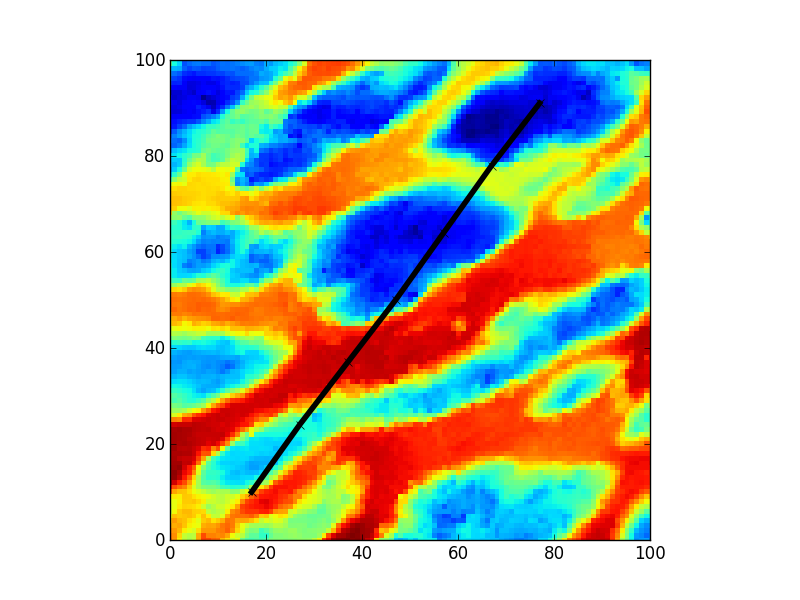
\includegraphics[scale=.5]{../data/illustration_recalage_baseline/plot_A_10_17_B_91_77_iteration_000.png}}
\only <2> {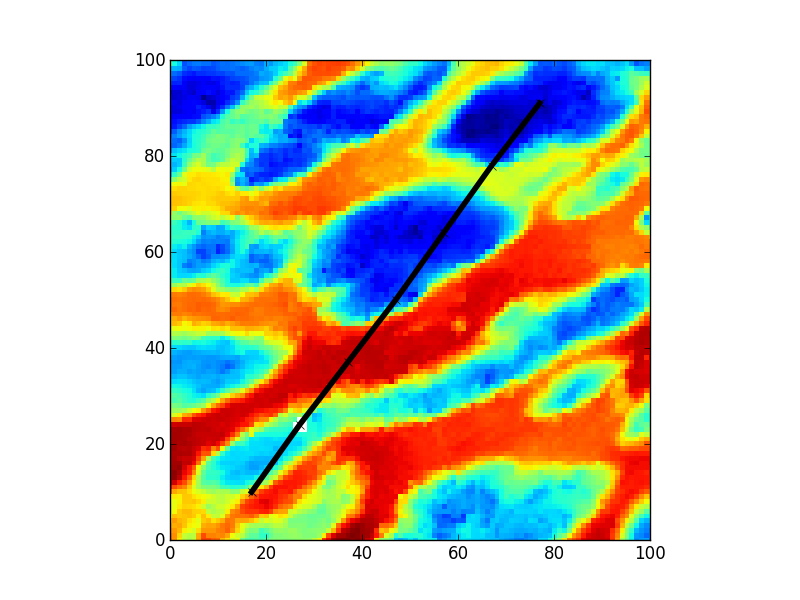
\includegraphics[scale=.5]{../data/illustration_recalage_baseline/plot_A_10_17_B_91_77_iteration_001.png}}
\only <3> {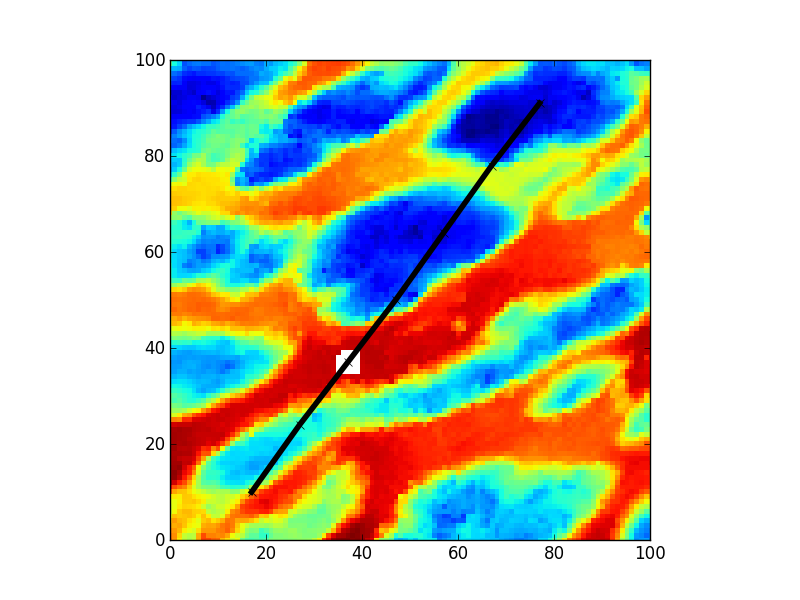
\includegraphics[scale=.5]{../data/illustration_recalage_baseline/plot_A_10_17_B_91_77_iteration_002.png}}
\only <4> {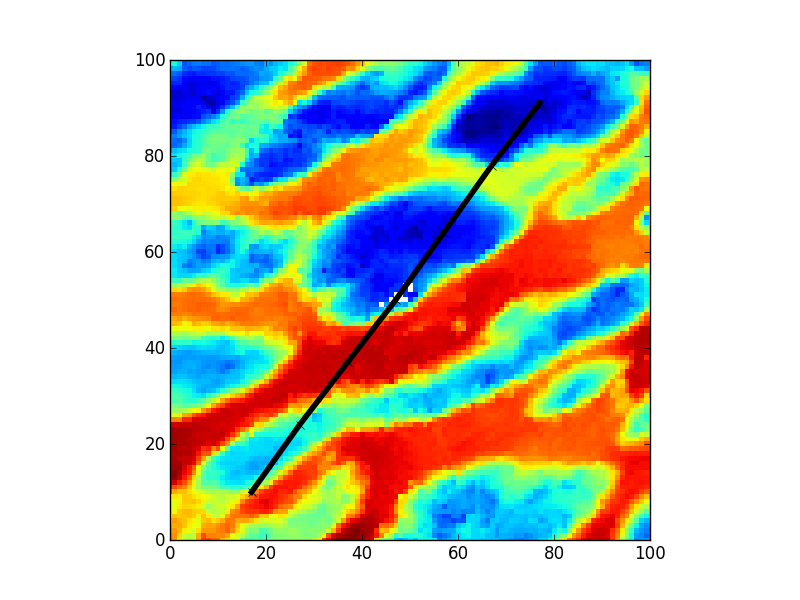
\includegraphics[scale=.5]{../data/illustration_recalage_baseline/plot_A_10_17_B_91_77_iteration_003.png}}
\only <5> {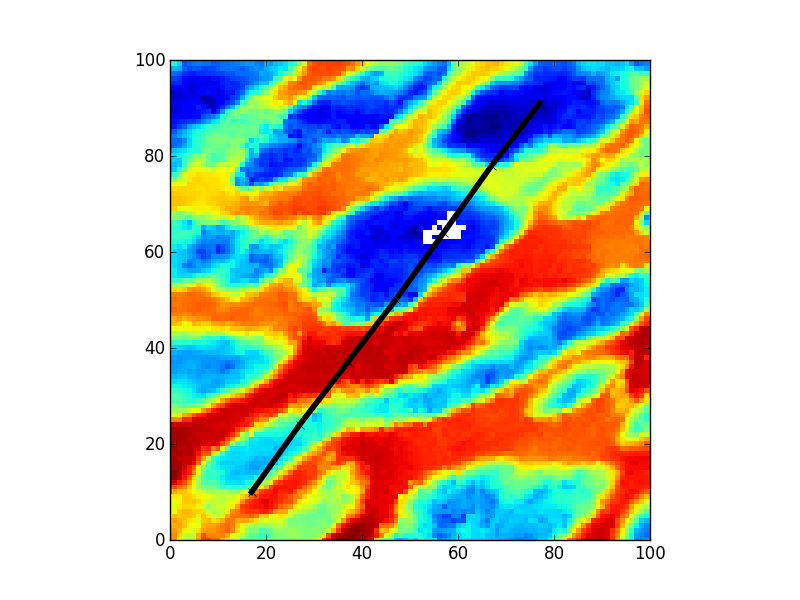
\includegraphics[scale=.5]{../data/illustration_recalage_baseline/plot_A_10_17_B_91_77_iteration_004.png}}
\only <6> {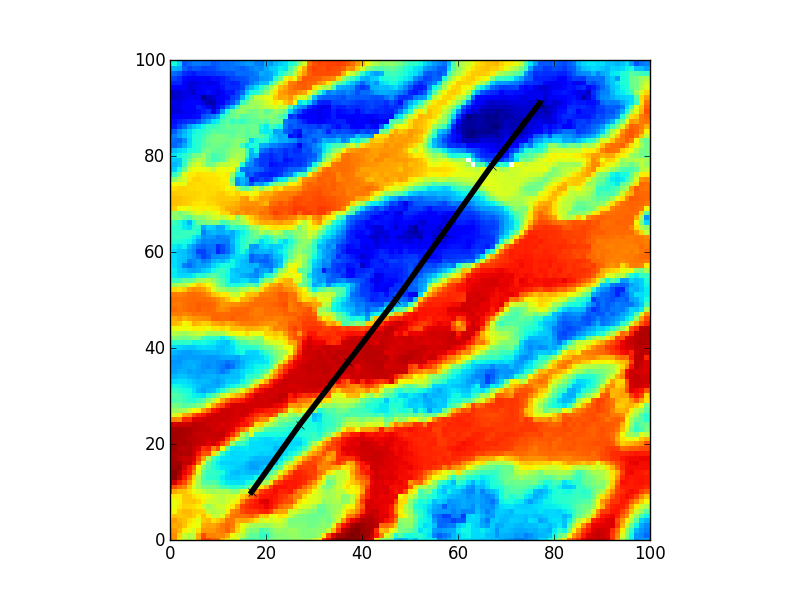
\includegraphics[scale=.5]{../data/illustration_recalage_baseline/plot_A_10_17_B_91_77_iteration_005.png}}
\only <7> {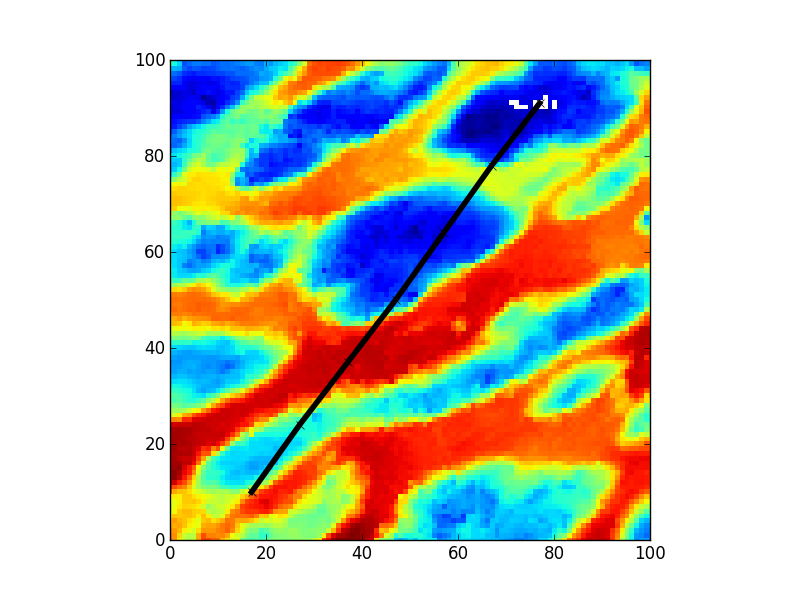
\includegraphics[scale=.5]{../data/illustration_recalage_baseline/plot_A_10_17_B_91_77_iteration_006.png}}
\end{overlayarea}
\end{frame}



%%%%%%%%%%%%%%%%%%%%%%%%%%%%%%%%%%%%%
\section{Optimisation de trajectoire}
\subsection{Gloutonne}
%%%%%%%%%%%%%%%%%%%%%%%%%%%%%%%%%%%%%%%

\begin{frame}

\frametitle{Stratégie gloutonne}


% Notre premier algorithme glouton donne une \textcolor{red}{bonne trajectoire} $\gamma_0$.\\
% ~\\
\textcolor{red}{Remarque :} Il faut trouver des \textcolor{blue}{forts gradients}, qui sont successivement "\textcolor{blue}{orthogonaux}" !\\




\begin{figure}[!h]
\begin{center}
\begin{tikzpicture}

    %% main box
    \draw (0,0) rectangle (10,6.3);

    \node at (5,3.5) {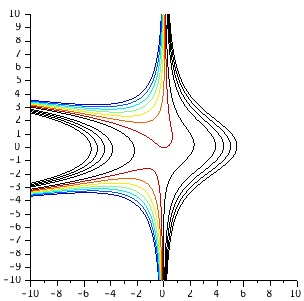
\includegraphics[scale = 0.5]{Images/LevelSet.jpg}};

    \only <1,2> {\fill [red] (7.5, 3) circle (0.2); \node[red] at (8.2, 3) {$J_{k-1}$};}

    \only <2> {
    \fill[red] (5.5, 2.7) circle (0.4);
    \draw[line width=1, ->] (7.5, 3) -> (5.5, 2.7);
    \node[red] at (6.2, 2) {$T(J_{k-1})$};}


    \only <3,4> {
    \fill[red, rotate around={50:(5.5, 2.7)}] (5.5,2.7) ellipse (0.4 and 0.15);     \node[red] at (5.7, 2.2) {$J_k$};
    }

    \only <3> {\draw[line width=1, ->] (5.5, 2.7) -> (6.5, 2); \node at (7.5, 2) {$\nabla H(A_{k})$};}

    \only <4> {
        \fill[red, rotate around={50:(6, 4)}] (6,4) ellipse (0.5 and 0.25);
        \draw[line width=1, ->] (5.5, 2.7) -> (6, 4);
    }
    \only <4> {
        \node[red] at (7, 4) {$T(J_k)$};
    }
    \only <5> {
        \fill[red, rotate around={50:(6, 4)}] (6,4) ellipse (0.1 and 0.25);
        \draw[line width=1, ->] (6, 4) -> (7, 5); \node at (8, 5) {$\nabla H(A_{k+1})$};
        \node[red] at (7, 4) {$J_{k+1}$};
    }

\end{tikzpicture}
\end{center}
\end{figure}



\end{frame}

%%%%%%%%%%%%%%%%%%%%%%%%%%%%%%%%%%%%%%%%%%



\begin{frame}

\frametitle{Algorithme glouton}

On en déduit une \textcolor{blue}{stratégie gloutonne} : \\
~\\
% \textcolor{red}{ALGORITHME :}\\
\begin{itemize}
    \item On pose $\gamma = [A]$, et $P = A$.
    \item Tant que $P \neq B$,
    \begin{itemize}
        \item Calculer $E_P = \{P', \ r_{\rm min} \le d(P, P') \le r_{\rm max}, \ d(P', B) < d(P, B) \}$.
        \item Si $B \in E_P$, $\gamma = [\gamma, B]$, $P = B$.
        \item Sinon, poser
        \[
            P_{\rm next} = \argmin \left\{ \Big| \nabla H(P') \wedge \nabla H(P) \Big|, P' \in E_P    \right\}
        \]
        puis $\gamma = [\gamma, P_{\rm next}]$, et $P = P_{\rm next}$.
    \end{itemize}
\end{itemize}

\textcolor{red}{Remarque :}
Les constantes $r_{\rm min}$ et $r_{\rm max}$ prennent en compte la vitesse minimale et maximale du sous-marin, et la fréquence d'échantillonnage !


\end{frame}


%%%%%%%%%%%%%%%%%%%%%%%%%%%%%%%%%%%%%%%%%%%

%%%%%%%%%%%%%%%%%%%%%%%%%%%%%%%%%%%%%%%%%%
\subsection{Dijkstra}
%%%%%%%%%%%%%%%%%%%%%%%%%%%%%%%%%%%%%%%%%%%

\begin{frame}

\frametitle{Stratégie globale}
La stratégie gloutonne est locale: on cherche un algorithme \textcolor{blue}{global}.\\
On considère les pixels de la carte comme des noeuds et on calcule le coût de passage de l'un à l'autre.
\begin{center}
\only<1>{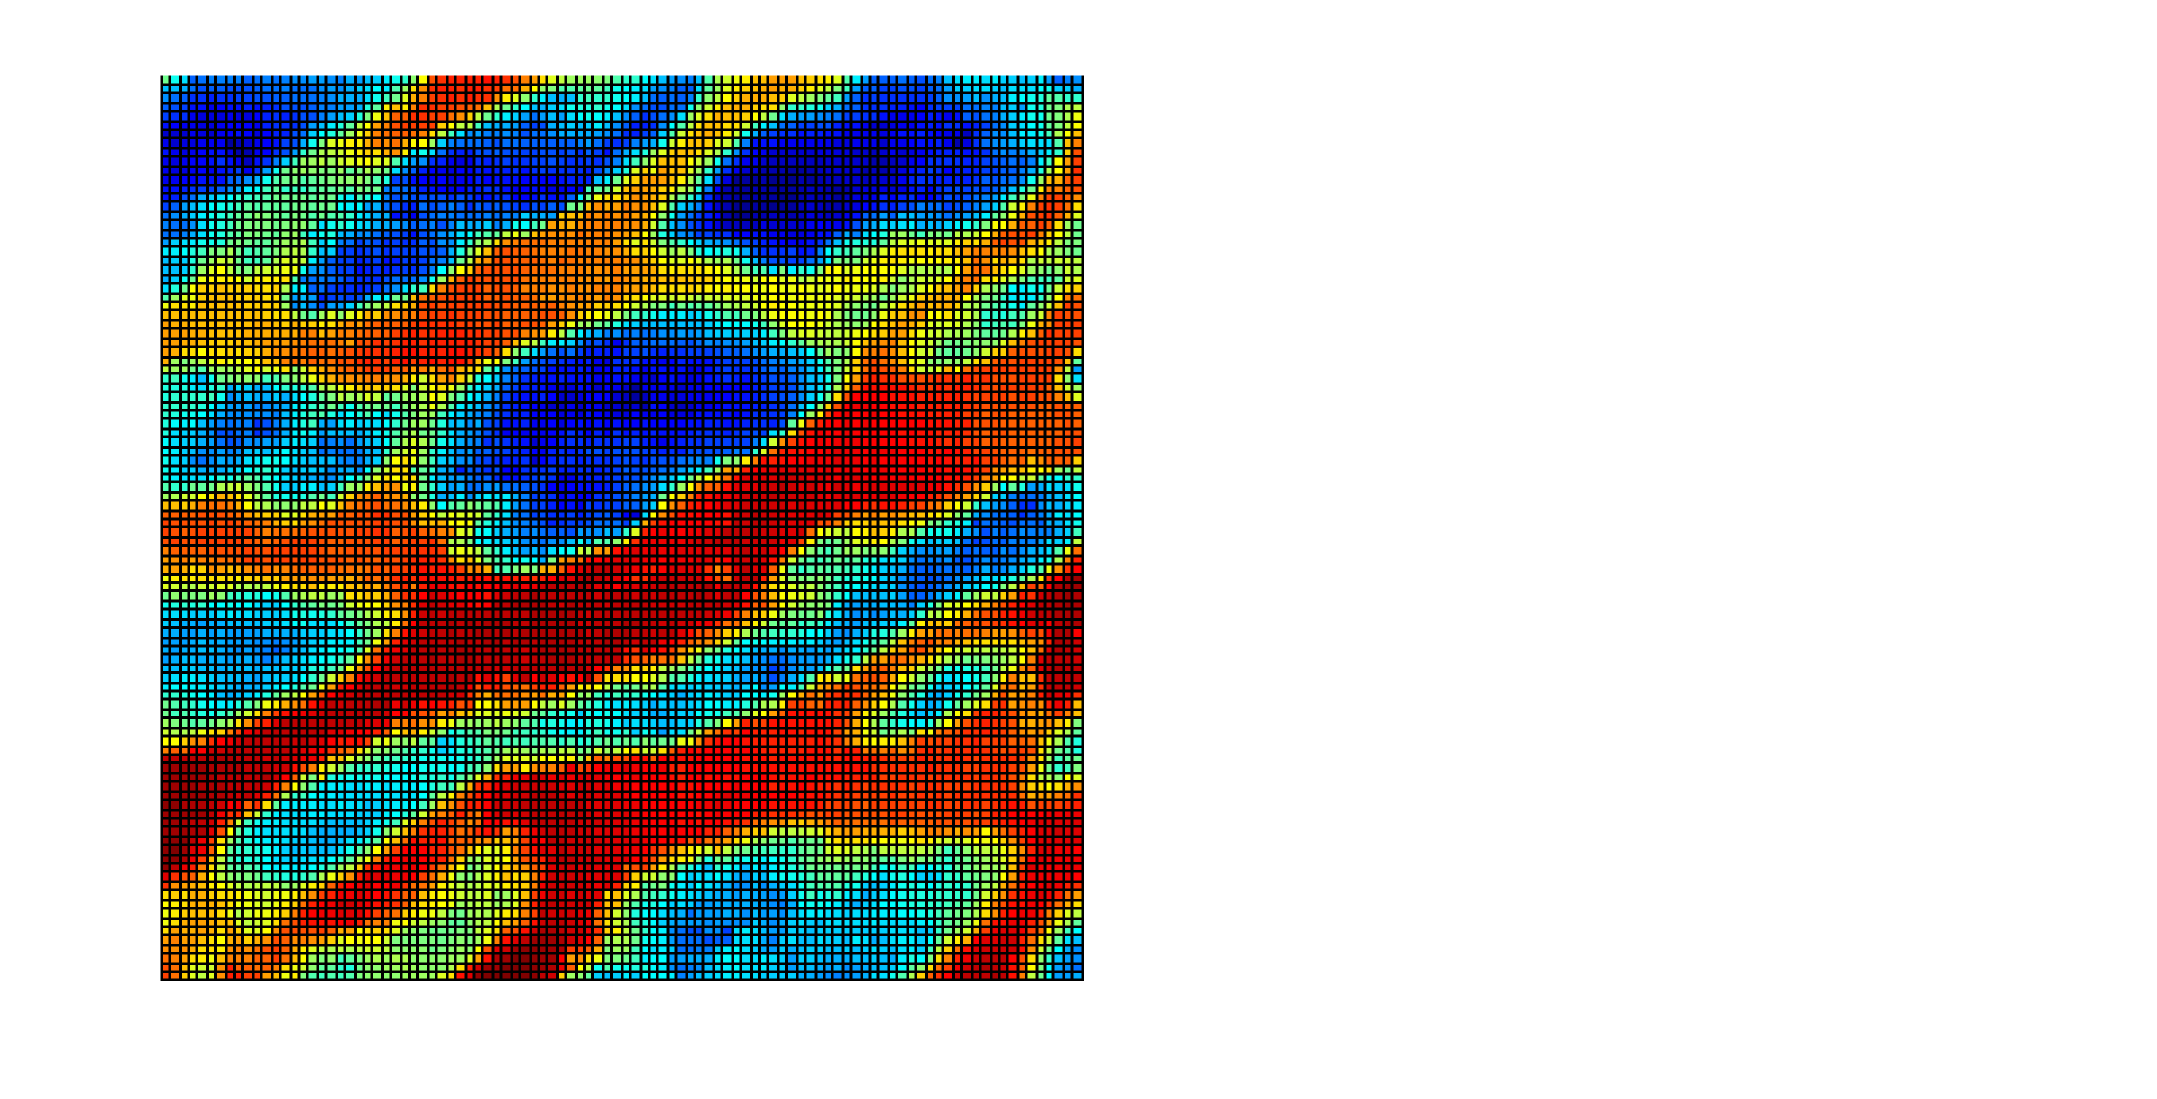
\includegraphics[width=.8\textwidth]{Images/morne_rouge_grid.png}}
\only<2>{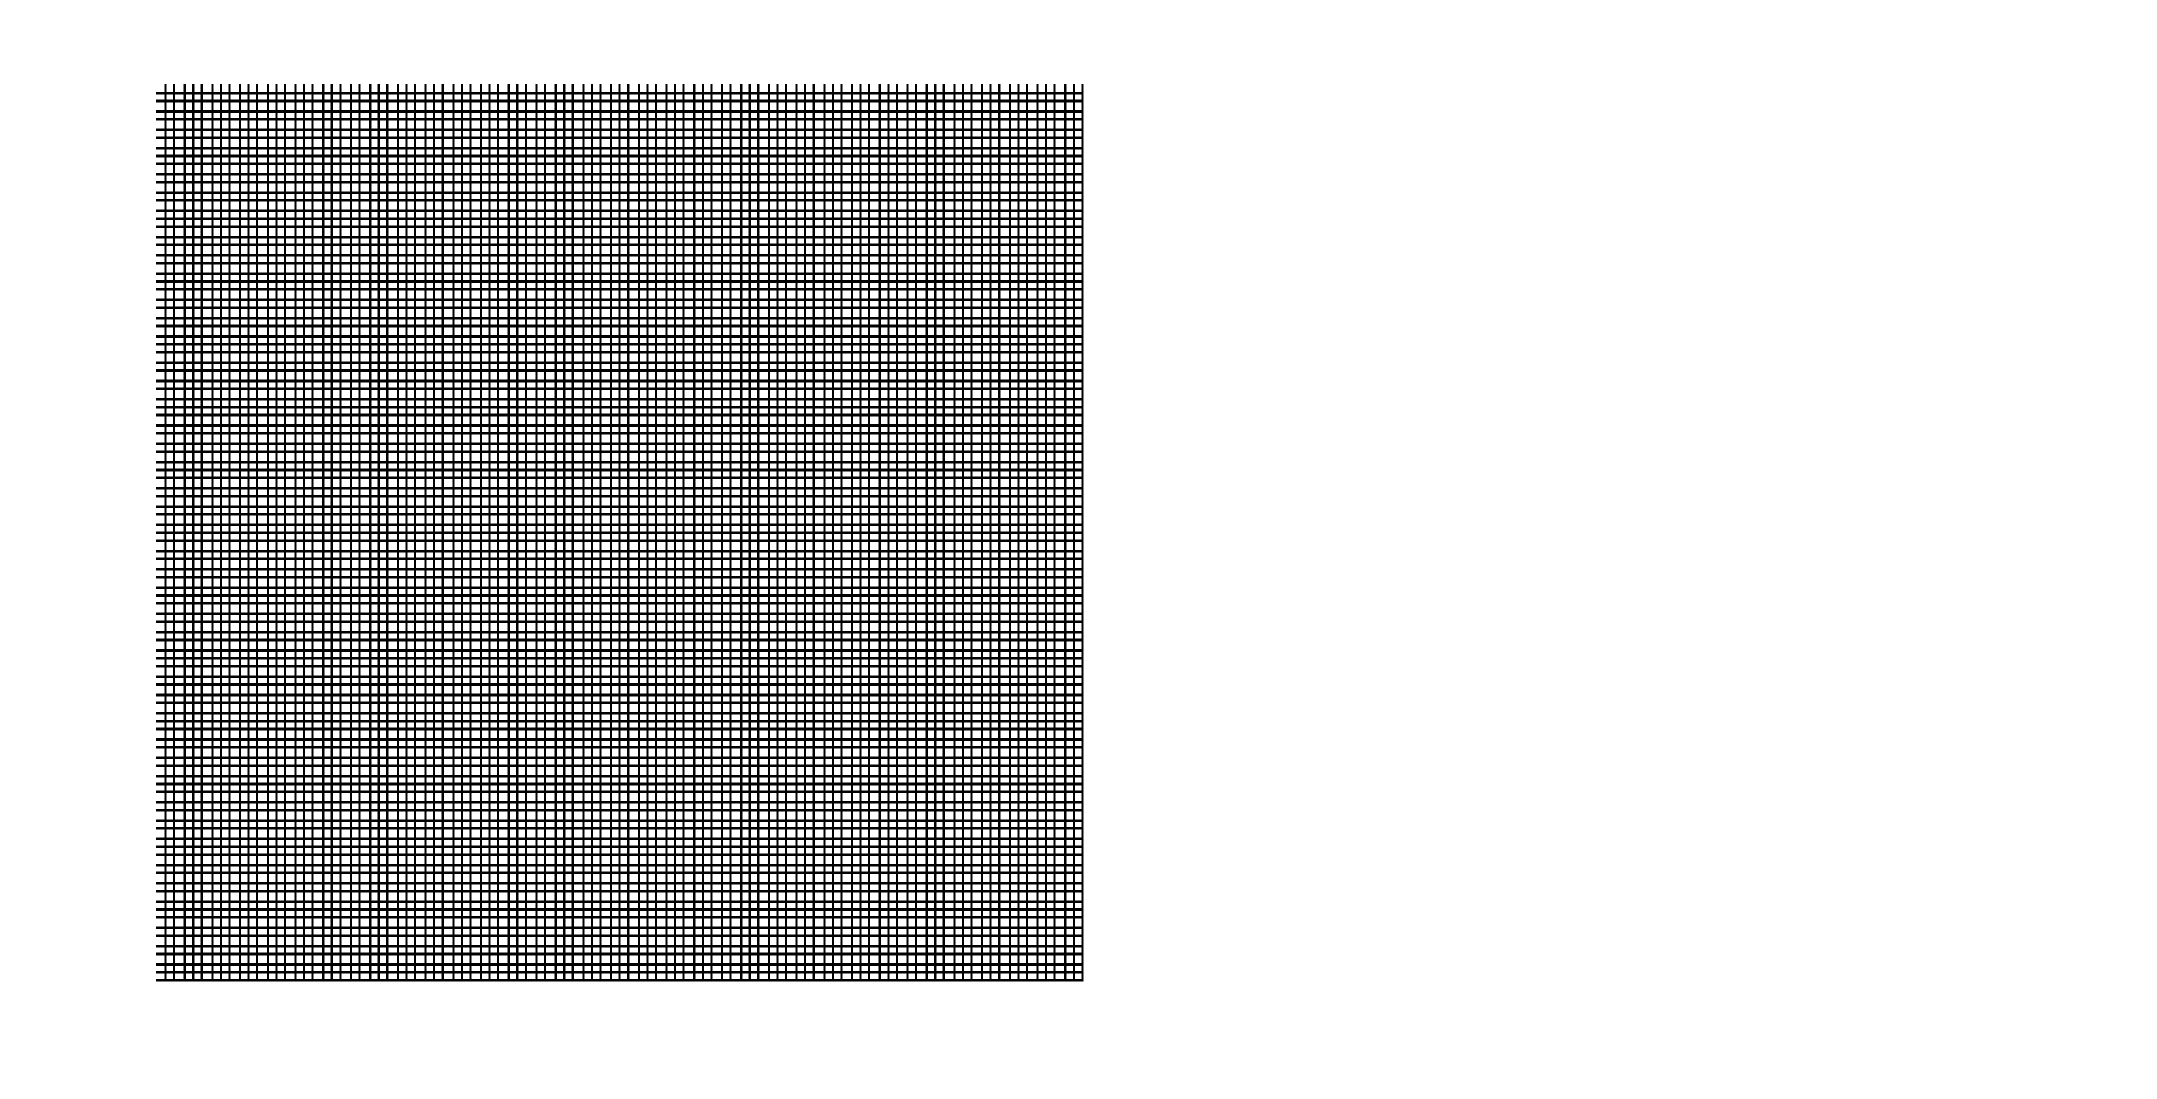
\includegraphics[width=.8\textwidth]{Images/morne_rouge_grid_only.png}}
\only<3>{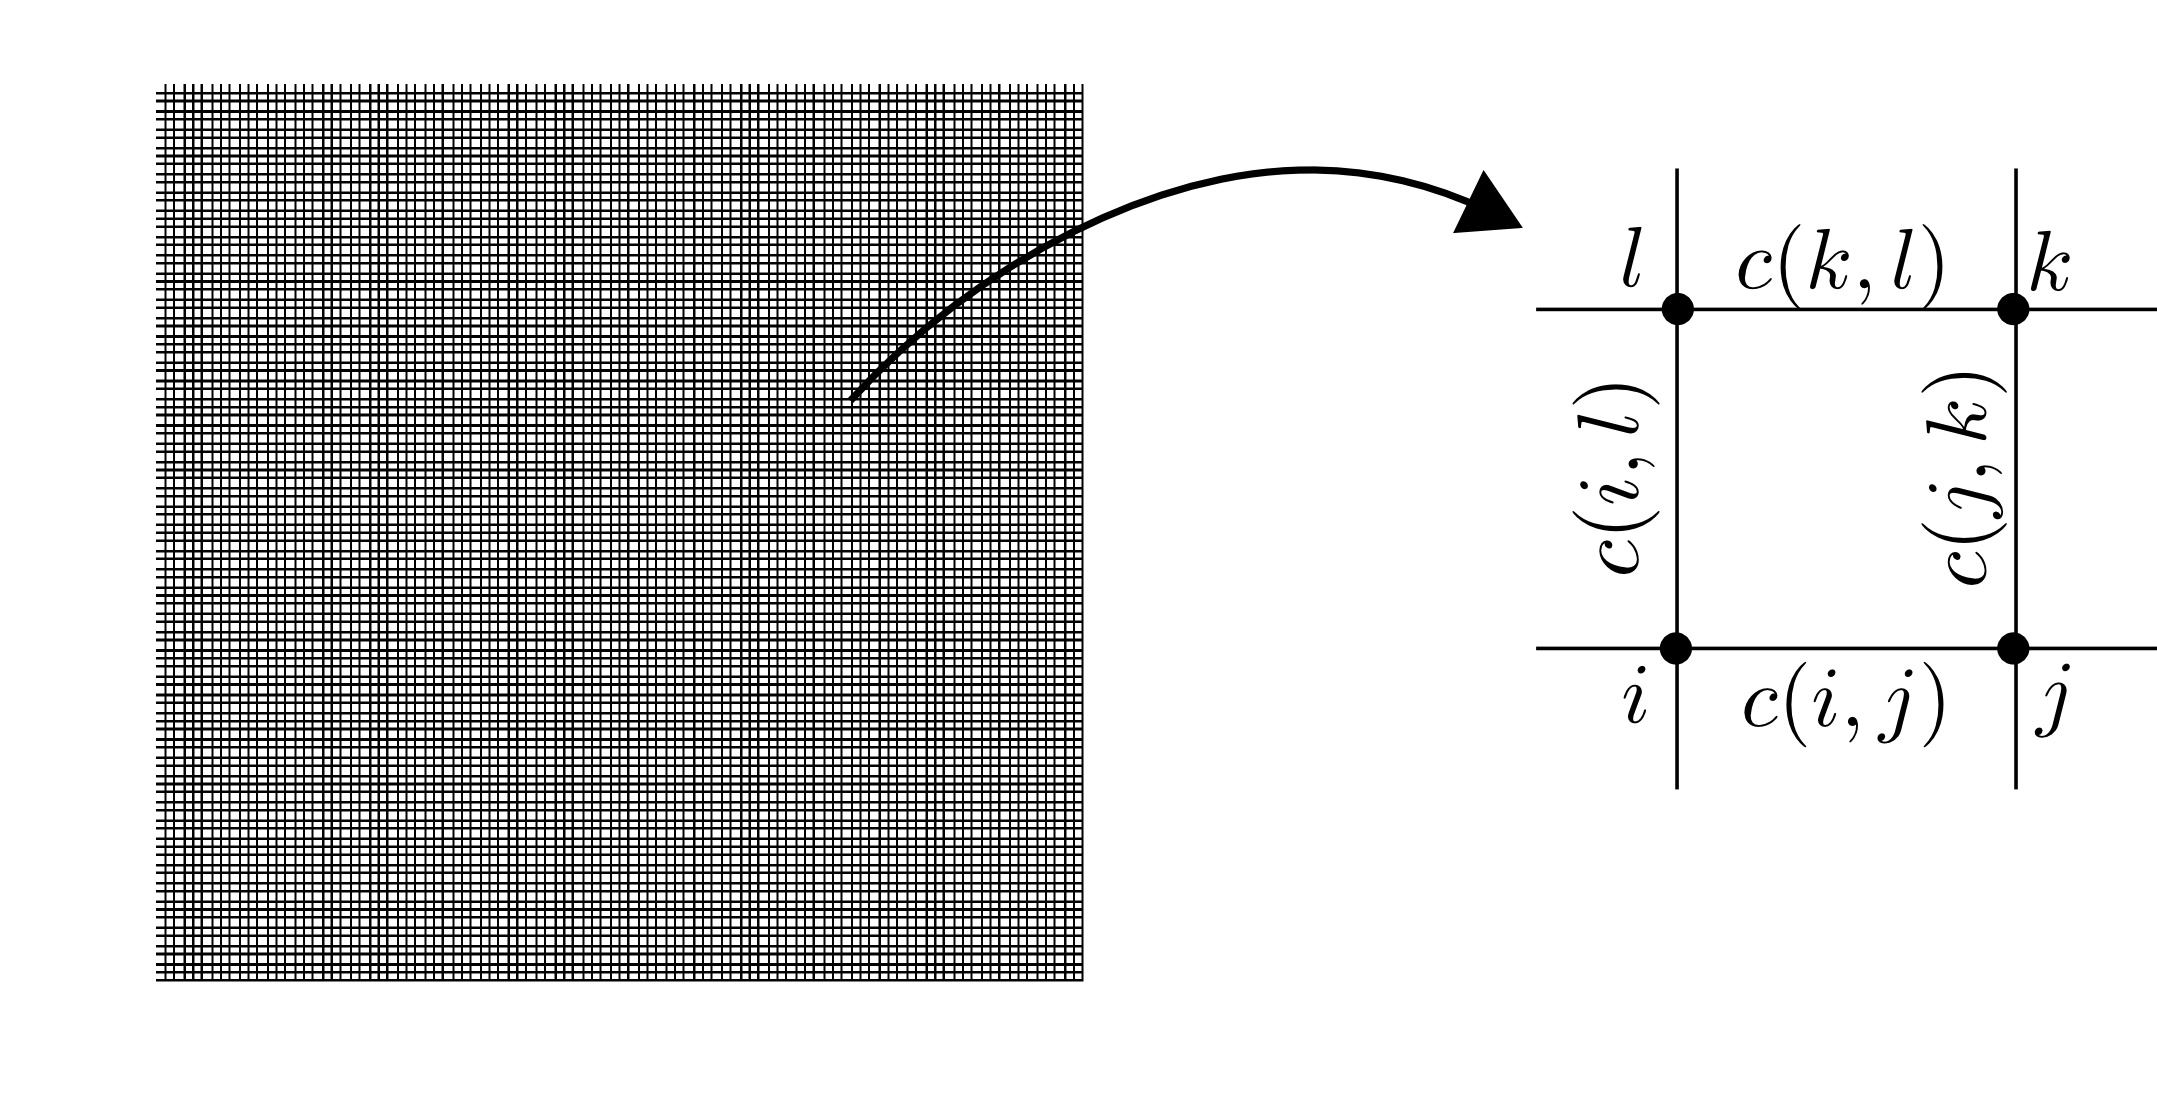
\includegraphics[width=.8\textwidth]{Images/network.png}}
\end{center}
En pratique, on définit
\begin{equation*}
  c(i,j) = \left( \left| \nabla H(i) \wedge \nabla H(j) \right| - \alpha \left( d(j,B) - d(i,B) \right) \right)^{-1} .
\end{equation*}


\end{frame}

\begin{frame}
\frametitle{Algorithme global}
On peut donc définir un nouvel algorithme\\
~\\
\begin{itemize}
\item Pour tout $(P, P')$ tels que
  \[
  r_{\rm min} \le d(P, P') \le r_{\rm max}, \ d(P', B) < d(P, B),
  \]
  on calcule $c(P,P')$.
\item On construit la \textcolor{blue}{matrice de coût} du graphe.
\item On applique l'algorithme de Dijkstra et on obtient la \textcolor{blue}{trajectoire du coût minimal} entre A et B.
\end{itemize}

\vfill
 % \textcolor{red} {\fontencoding{U}\fontfamily{futs}\selectfont\char 66\relax}
Croissance en $ N^2(r_{\rm max} - r_{\rm min})^2$ du coût de l'algorithme : trop lent pour des cartes de taille elevée.
\end{frame}
\subsection{Résultats}
\begin{frame}{Autre version}
\begin{center}
%\begin{tikzpicture}
%\draw[gray] (0,0) grid[xstep=0.125,ystep=0.125] (1,1);
%\end{tikzpicture}
\begin{tikzpicture}[scale=0.5]
\draw[gray] (0,0) grid[xstep=0.125,ystep=0.125] (1,1);
%\draw[gray] (0,0) -- (1,1);
%\draw[gray] (0,0.125) -- (0.875,1);
%\draw[gray] (0,0.25) -- (0.75,1);
%\draw[gray] (0,0.375) -- (0.625,1);
%\draw[gray] (0,0.5) -- (0.5,1);
%\draw[gray] (0,0.625) -- (0.375,1);
%\draw[gray] (0,0.75) -- (0.25,1);
%\draw[gray] (0,0.875) -- (0.125,1);
%\draw[gray] (0.125,0) -- (1,0.875);
%\draw[gray] (0.25,0) -- (1,0.75);
%\draw[gray] (0.375,0) -- (1,0.625);
%\draw[gray] (0.5,0) -- (1,0.5);
%\draw[gray] (0.625,0) -- (1,0.375);
%\draw[gray] (0.75,0) -- (1,0.25);
%\draw[gray] (0.875,0) -- (1,0.125);
\draw (0,0) grid (8,8);
%\draw[|-|,>=latex] (-0.5,2) -- (-0.5,3);
%\draw node[left] at (-0.5,2.5) {$H$};
\draw[->,>=latex] (-0.35,0.3) -- (0.2,0.3);
\draw node[left] at (-0.25,0.3) {$C$};
\end{tikzpicture}
\end{center}




\begin{itemize}
\item Soit $r\in (0,1)$. Dans chaque sous partie $C$ , sélectionner l'ensemble des points $P$ tels que $\|\nabla h(P)\|\geq \|\nabla h\|_{\mathit{L}^\infty(C)}(1-r)$.
\item Coût $c(P,Q)=c(\{P,Q\})$ pour tout $Q\in E_P$.
\end{itemize}
\end{frame}
\begin{frame}[Résultats]
  \frametitle{Résultats}
\only<1>{\begin{tabular}{cc}
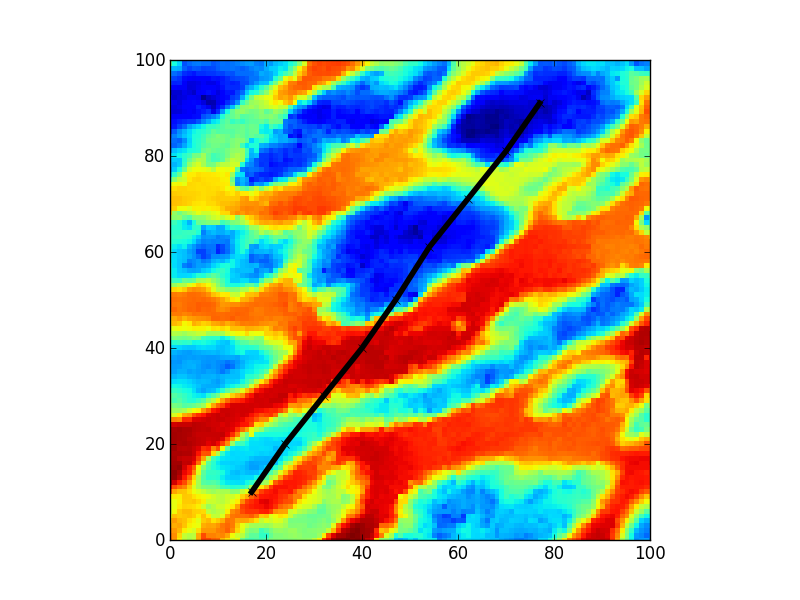
\includegraphics[scale=0.25]{../data/baseline/plot_A_10_17_B_91_77_iteration_000.png} &
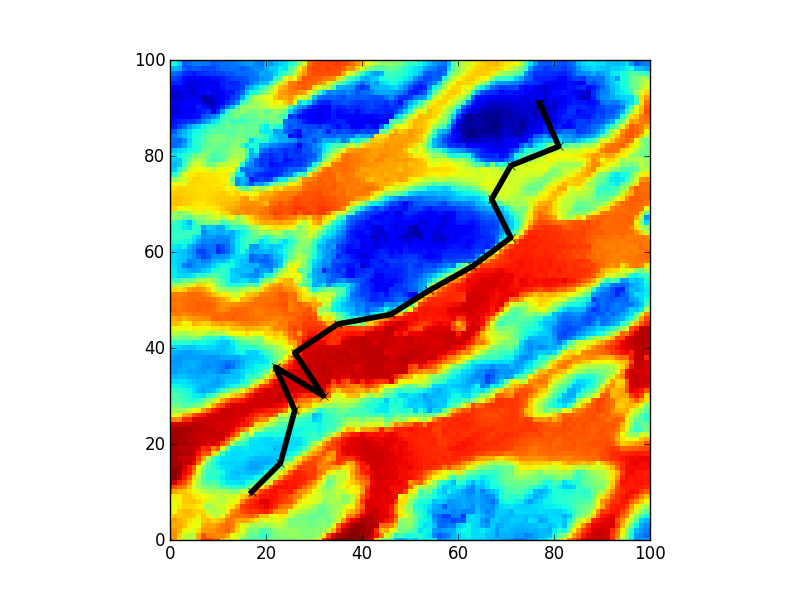
\includegraphics[scale=0.25]{../data/greedy/plot_A_10_17_B_91_77_iteration_000.png} \\
%cost=91&cost=\\
&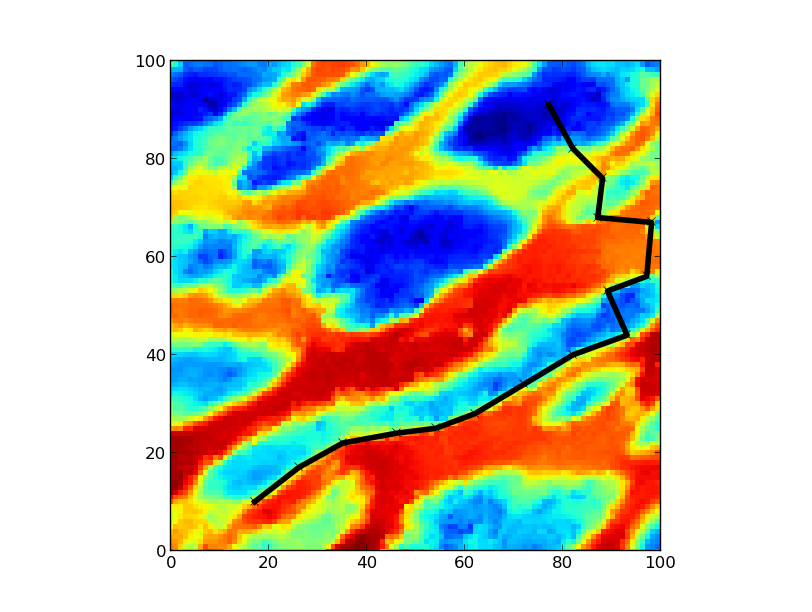
\includegraphics[scale=0.25]{../data/None_dijkstra/plot_A_10_17_B_91_77_iteration_000.png} \\
%&cost=26\\
\end{tabular}
}
%\only<2>{\begin{tabular}{cc}
%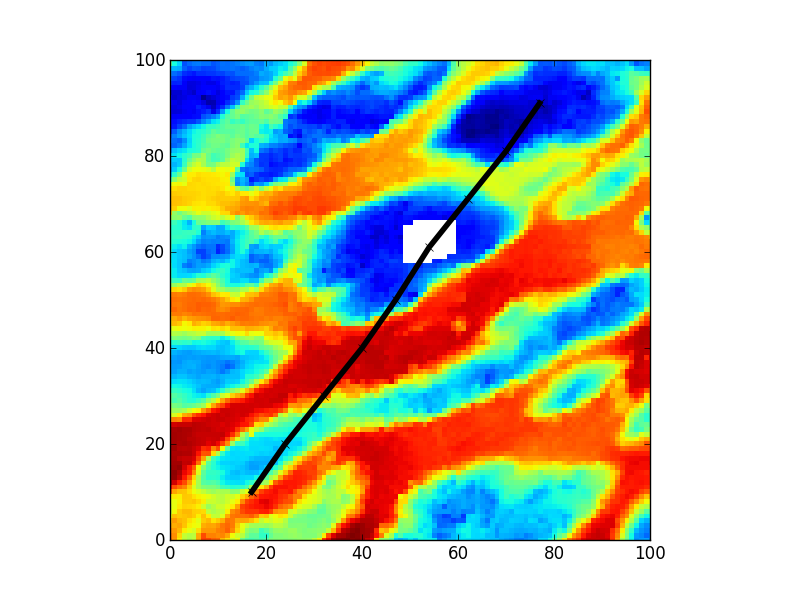
\includegraphics[scale=0.25]{../data/baseline/plot_A_10_17_B_91_77_iteration_005.png} &
%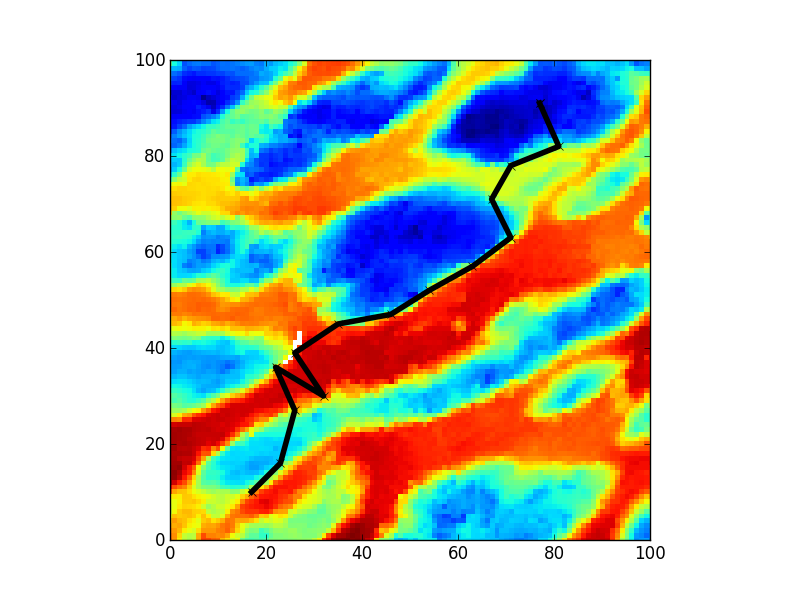
\includegraphics[scale=0.25]{../data/greedy/plot_A_10_17_B_91_77_iteration_005.png} \\
%cost=91&cost=\\
%&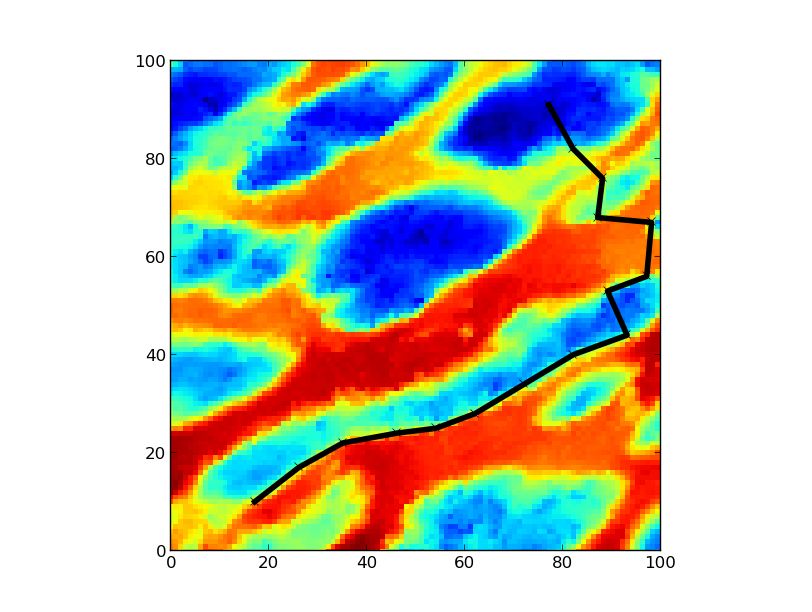
\includegraphics[scale=0.25]{../data/None_dijkstra/plot_A_10_17_B_91_77_iteration_005.png} \\
%&cost=26\\
%\end{tabular}
%}
%\only<3>{\begin{tabular}{cc}
%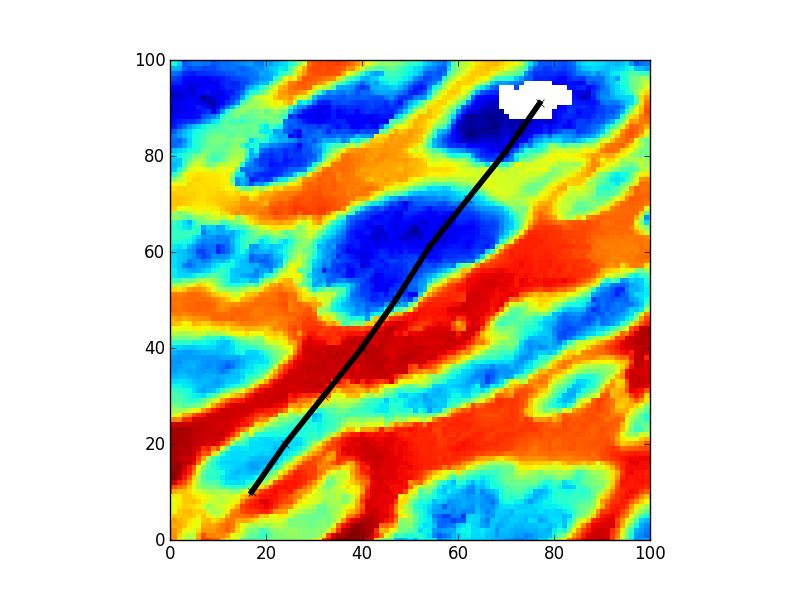
\includegraphics[scale=0.25]{../data/baseline/plot_A_10_17_B_91_77_iteration_008.png} &
%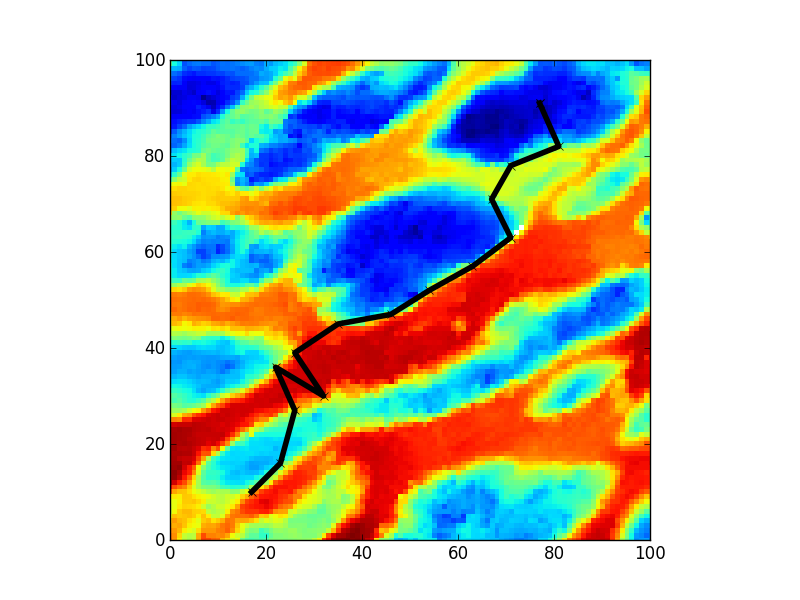
\includegraphics[scale=0.25]{../data/greedy/plot_A_10_17_B_91_77_iteration_010.png}\\
%cost=91&cost=\\
%&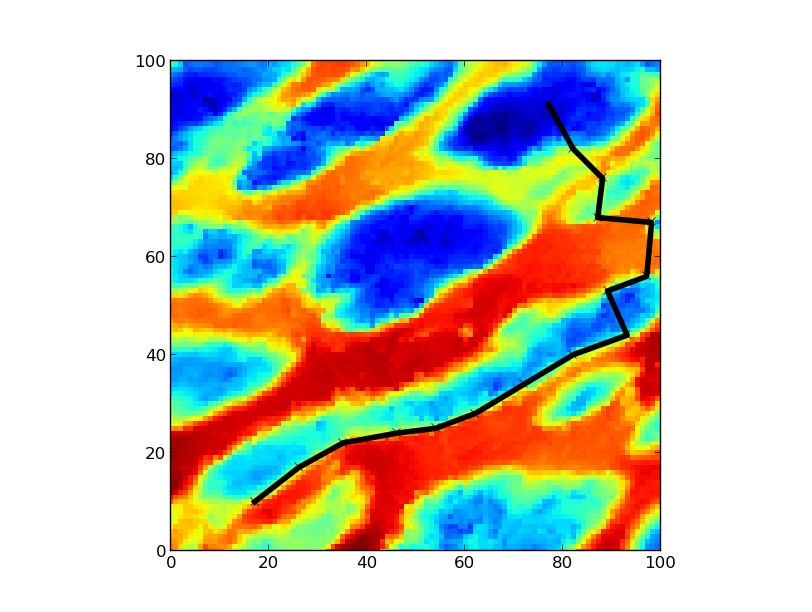
\includegraphics[scale=0.25]{../data/None_dijkstra/plot_A_10_17_B_91_77_iteration_010.png}  \\
%&cost=26\\
%\end{tabular}
%}
\only<2>{\begin{tabular}{cc}
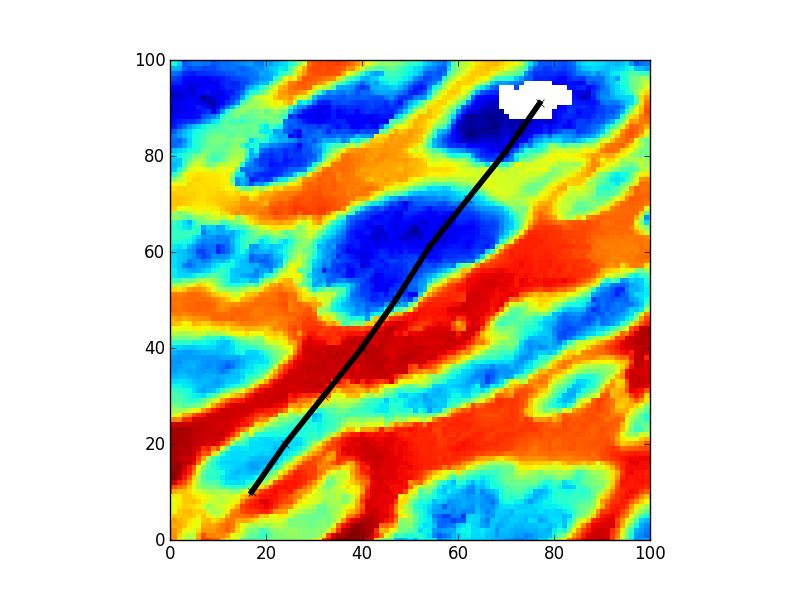
\includegraphics[scale=0.25]{../data/baseline/plot_A_10_17_B_91_77_iteration_008.png} &
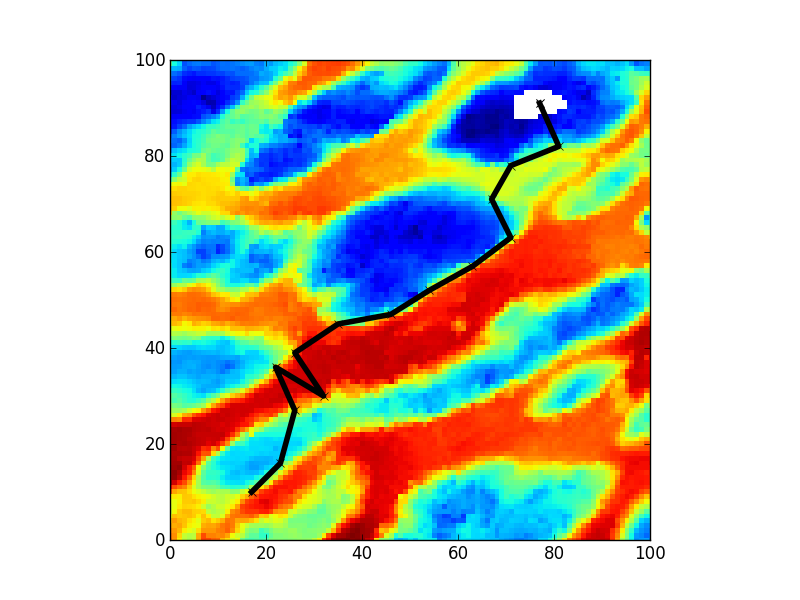
\includegraphics[scale=0.25]{../data/greedy/plot_A_10_17_B_91_77_iteration_015.png} \\
%cost=91&cost=\\
&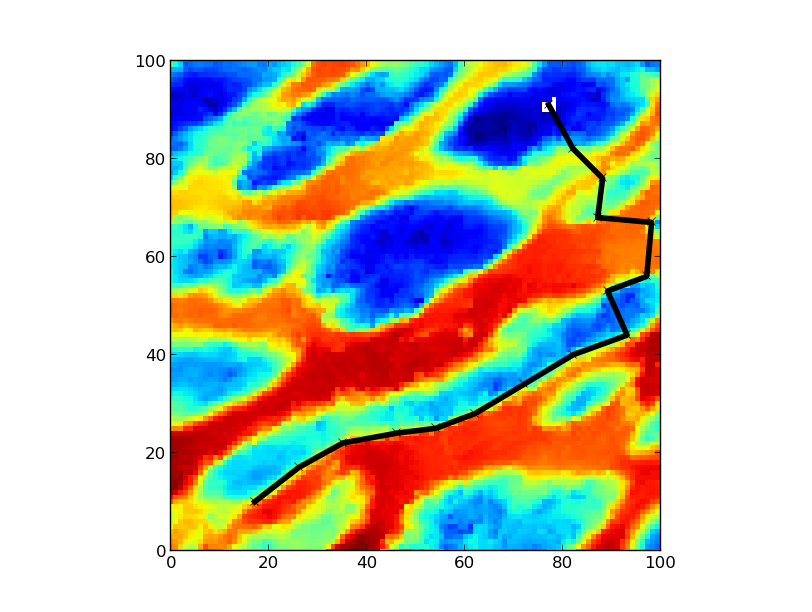
\includegraphics[scale=0.25]{../data/None_dijkstra/plot_A_10_17_B_91_77_iteration_015.png} \\
%&cost=26\\
\end{tabular}
}
\end{frame}
\section{Pistes continues}


%%%%%%%%%%%%%%%%%%%%%%%%%%%%%%%%%%%%%%%%%%%

%%%%%%%%%%%%%%%%%%%%%%%%%%%%%%%%%%%%%%%%%%%

% \begin{frame}

% \frametitle{Variantes et énoncé sous forme discrète}


% \textcolor{red}{Variantes :}
% \begin{itemize}
% 	\item Le temps final $T$ peut-être libre,
% 	\item On peut vouloir minimiser \textcolor{red}{l'incertitude globale}, au lieu de l'incertitude finale,
% 	\item On peut vouloir rajouter des contraintes sur $\gamma_0$, par exemple
% 	\[
% 		\forall \ 0 \le t \le T, \quad \left\| \gamma'(t) \right\|_\infty \in [v_{\rm min}, v_{\rm max}].
% 	\]
% \end{itemize}

% \textcolor{red}{En pratique, toutes les données sont discrètes :}
% \begin{itemize}
% 	\item Le sous-marin réel prend des mesures avec une certaine fréquence (1Hz, ici, 0.1 Hz)
% 	\item La carte est "pixellisée" (1 pixel = 1 mètre)
% \end{itemize}

% \begin{center}
% \textcolor{red}{On va chercher des stratégies d'optimisation pour des problèmes discrets.}
% \end{center}

% \end{frame}


\begin{frame}
  \frametitle{Modèle jouet}
  On cherche à aller sur des zones de grande pente:
  \begin{align*}
    c(\gamma) = -\int_{t=0}^{1} |\nabla h(\gamma(t))|^{2}  dt
  \end{align*}

  Mal posé (les suites minimisantes se localisent sur les maxima de
  $\nabla h$) : régularisation~?
  
\begin{align*}
  c(\gamma) =  \int_{t=0}^{1} a |\gamma'(t)|^{2} - b |\nabla
  h(\gamma(t))|^{2} dt
\end{align*}

Bien posé~? Minimiseurs~? Comment prendre en compte l'heuristique que
$\gamma$ doit alterner les directions de $\nabla h$ pour se localiser~?

% \begin{align*}
%   c(\gamma) =  \int_{t=0}^{1} a |\gamma'(t)|^{2} - b |\nabla
%   h(\gamma(t)) \cdot \gamma'(t)| dt
% \end{align*}

\end{frame}
\begin{frame}
  \frametitle{Un modèle un peu plus complexe}
Modèle effectif pour les incertitudes en $x$ et $y$ $\sigma_{x}$ et
$\sigma_{y}$ :
\begin{align*}
  c(\gamma) &= \sigma_{x}(1) + \sigma_{y}(1), \text{ où}\\
  \dot \sigma_{x} &= a - b \sigma_{x} (\partial_{x} h(\gamma(t)))^{2}\\
  \dot \sigma_{y} &= a - b \sigma_{y} (\partial_{y} h(\gamma(t)))^{2}.
\end{align*}
Amortissement exponentiel vers un point d'équilibre $\sigma_{x} \sim
1/(\partial_{y} h(\gamma(t)))^{2}$. Sous la forme générale d'un
contrôle optimal. Problème : modèle non isotrope (trajectoires
diagonales~?)

Généralisation : représenter l'incertitude par une matrice SDP $A$. Si
on pose $G = \nabla h \nabla h^{T}$,
\begin{align*}
  \dot A = a A - b \sqrt G A \sqrt G.
\end{align*}
On modifie les incertitudes dans la direction $\nabla h$, on n'y
touche pas dans $\nabla h^{\perp}$. Problème : $A$ ne reste
pas forcément SDP. Y a-t-il une bonne généralisation~?
\end{frame}

\section{Pistes probabilistes}
\begin{frame}
  \frametitle{Modélisation des incertitudes}
\begin{itemize}
\item Sources d'incertitude : précision de l'accéléromètre, erreurs
  d'intégration (fréquence finie), erreur numérique (stockage en
  virgule flottante)
\item Dérive de l'estimation de position
\item Modélisation délicate
\item Si on fait une erreur initiale sur l'accélération, dérive en
  $t^{2}$
\item Si on fait une erreur initiale sur la vitesse, dérive en
  $t$
\item Compensation des erreurs~? Marche aléatoire, dérive en $\sqrt t$
 ~? $t^{3/2}$~? $t^{5/2}$~?
\item Non trivial en pratique
\end{itemize}
\end{frame}

\begin{frame}
  \frametitle{Modélisation probabiliste}
  \begin{itemize}
  \item Une approche par intervalles néglige la compensation des erreurs
    et est trop pessimiste. Modèle probabiliste~?
  \item Soit $(x_{0}, x_{1} \dots, x_{N})$ le chemin suivi par le
    sous-marin, supposé exact.
  \item Soit $X_{n}$ la position estimée du sous-marin. Loi de
    $X_{n+1}$~?
  \item Sans bathymétrie, on met à jour la position avec le vecteur
    vitesse $v_{n} = x_{n+1} - x_{n}$, entaché (pour simplifier) d'une erreur aléatoire
    $\varepsilon_{v} \sim N(0, \sigma_{v})$
  \item La bathymétrie nous donne $h(X_{n+1}) = h(x_{n+1}) +
    \varepsilon_{h}$, avec une erreur $\varepsilon_{h} \sim N(0, \sigma_{h})$
  \end{itemize}

  \begin{center}
  \boxed{\mbox{$X_{n+1} \sim L(X_{n} + v_{n} + \varepsilon_{v} \;\Big|\;
    h(X_{n} + v_{n} + \varepsilon_{v}) = h(x_{n+1}) + \varepsilon_{h})$}}
  \end{center}
\end{frame}
\begin{frame}
  \frametitle{Modélisation probabiliste}
  \begin{center}
  \boxed{\mbox{$X_{n+1} \sim L(X_{n} + v_{n} + \varepsilon_{v} \;\Big|\;
    h(X_{n} + v_{n} + \varepsilon_{v}) = h(x_{n+1}) +  \varepsilon_{h})$}}
  \end{center}

  En notant formellement $P(X=x)$ pour la densité de $X$ en $x$,
  \begin{align*}
    P(X_{n+1} = x) &= P(X_{n} + v_{n} + \varepsilon_{v} = x \;\Big|\;
    h(X_{n} + v_{n} + \varepsilon_{v}) = h(x_{n+1}) + 
                     \varepsilon_{h})\\
    &= \frac 1 N P(X_{n} + v_{n} + \varepsilon_{v} = x \cap
    h(X_{n} + v_{n} + \varepsilon_{v}) = h(x_{n+1}) + \varepsilon_{h})\\
    &= \frac 1 N P(X_{n} + v_{n} + \varepsilon_{v} = x) \; P(h(x) = h(x_{n+1}) + \varepsilon_{h}),
  \end{align*}
  où $N$ est choisi pour normaliser $X_{n+1}$.

  On calcule $P(h(x) = h(x_{n+1}) + \varepsilon_{h})$ (facile si
  $\varepsilon_{h}$ est gaussienne), on calcule $P(X_{n} + v_{n} +
  \varepsilon_{v} = x)$ (translation et convolution), on multiplie et on
  normalise. En théorie bien plus précis que l'approche par boites,
  mais quel traitement des incertitudes de vitesse~? Lien avec les
  filtres de Kalman~?
\end{frame}


\section{Conclusion}
\begin{frame}
\frametitle{Conclusion (ce qu'on a fait)}
\begin{itemize}

\item Comprendre et ``mathématiser'' le problème:
\begin{itemize}
\item Traduction du problème dans un langage mathématique grâce aux
  précisions de l'encadrant.
\item Développement d'un algorithme de recalage pour affiner l'intuition.
\item Traduction des données physiques (vitesse, carte bathymétrique )
  en conditions algorithmiques/mathématiques : couronne d'admissibilité,
  choix d'une direction de fort gradient.
\end{itemize}

\item Proposition de deux algorithmes discrets testés sur les
  cartes fournies :
\begin{itemize}
\item Stratégie gloutonne, locale et incrémentale, d'après les données
  physiques (gradient, distance, vitesse).

\item Stratégie globale basée sur un graphe décrivant
  les relations entre des points d'intérêts de la carte. La
  trajectoire de coût minimal est trouvée grâce à l'algorithme de Dijkstra.
\end{itemize}
\end{itemize}
\end{frame}

\begin{frame}
\frametitle{Conclusion (ce qu'on voudrait faire)}
\begin{itemize}
  \item Modélisation continue (modèle intégral, contrôle d'équations
    différentielles)
  \item Modélisation probabiliste (calcul de lois)
\end{itemize}
\end{frame}

\section{Bibliographie et ouvertures}
\begin{frame}

\frametitle{Quelques pistes bibliographiques}

\begin{itemize}

\item S.Barkby, S.B. Williams O.Pizarro, M.Y. Jakuba
  (2006). Amélioration d'une carte existante lors de la
  navigation. Contrôle avec une méthode de SLAM et un filtre de Rao.

\item D.Wettergreen (2008). Repositionnement sous l'eau. Découpe du
  volume à l'aide d'un \textit{octree}, et filtre de Kalman.

\item E.Galceran \& M.Carreras (2013) : article de review en CPP
  (\textit{Coverage Path Planning}). Déterminer le chemin passant par
  les points d'un volume (une aire) tout en évitant les obstacles
  éventuels. Algorithme de \textit{slicing}. Applications en
  bathymétrie.

\item E. Galceran, R. Campos N.Palomeras, D. Ribas, M. Carreras \&
  P. Ridao (2014). Trajectoire pour la cartographie du
  domaine. Séparation des régions selon le module du gradient. Régions
  de gradient fort traitées par un algorithme de \textit{slicing},
  autres régions traitées par l'algorithme de Boutrosphedon.
\end{itemize}

\end{frame}

\end{document}
